% Preview source code

%% LyX 2.1.1 created this file.  For more info, see http://www.lyx.org/.
%% Do not edit unless you really know what you are doing.
\documentclass[english]{article}
\usepackage[latin9]{inputenc}
\usepackage{float}
\usepackage{amstext}
\usepackage{graphicx}

\makeatletter

%%%%%%%%%%%%%%%%%%%%%%%%%%%%%% LyX specific LaTeX commands.
\newcommand{\lyxmathsym}[1]{\ifmmode\begingroup\def\b@ld{bold}
  \text{\ifx\math@version\b@ld\bfseries\fi#1}\endgroup\else#1\fi}

%% Because html converters don't know tabularnewline
\providecommand{\tabularnewline}{\\}

\makeatother

\usepackage{babel}
\begin{document}

\title{A Pedestrian Simulation }


\author{Castiglione Gonzalo, Agustin Marseillan, Daniel Parisi}
\maketitle
\begin{abstract}
En este paper se presenta un nuevo método para simular peatónes virtuales
basado en el modelo de la fuerza social. En el modelo presentado,
cada peatón posee un punto movil frente a el y camina siempre hasta
este. Este punto representa un objetivo a corto plazo que se debe
cumplir. Cada peatón se encarga de mover este punto según a donde
necesite llegar. 
\end{abstract}
keywords:

pedestrian, collision avoidance, future, force model

\pagebreak{}


\section{Introducción}

// Daniel tiene ya preparada una introducción\\


El transito de personas es un factor de suma importancia en el análisis
y diseño de instalaciones tales como edificios públicos, peatónales,
estaciones de trenes, entre otros. 

// Hace mucho tiempo que se viene estudiando a las personas en grupo
y se sabe que 

// Existen efectos de comportamiento colectivos de auto organización
tales como cuellos de botellas, formaciones en filas, bloqueos. 

// Decir porque una simulación de peatónes es útil para estas situaciones.\\


Analizar estructuras de transito de peatónes usando los cambios propuestos
para el modelo de la fuerza social. Implementar una interfaz gráfica
para poder visualizar los resultados de cambiar el modelo y cada uno
de los parámetros


\section{Formulacíon del modelo}

A continuación se presentan los efectos que van a determinar el movimiento
de un peatón:
\begin{enumerate}
\item El peatón desea alcanzar su objetivo a largo plazo de la manera mas
cómoda posible. Por lo tanto va a intentar alcanzarlo sin tener que
tomar desvios innecesarios, por ejemplo el camino mas corto.
\item El movimiento del peatón se ve influenciado por otros peatones. Dependiendo
de la distancia con la que se encuentre de otro peatón y la trayectoria
que se pueda predecir de este último, un peatón va a sentir la necesidad
de realizar cambios a la ruta deseada a fin de evitar colisiones.
Es por este efecto que el peatón va a necesitar recalcular su trayectoria
según nuevos peatones aparecen en su campo de visión.
\item La velocidad de movimiento se ver influenciada según necesidades o
estados de ánimo del peatón en cuestión.
\end{enumerate}
Para representar los efectos presentados, un peatón se encuentra definido
como según se especifica a continuación: 
\begin{itemize}
\item Area circular 


Representa el área física y espacio personal ocupado. El radio del
círculo es generado aleatoriamente a fin de representar peatónes diferentes.
El rango de valores se distribuye uniformemente en el intervalo $[0.25,0.29]$
$[cm]$.

\item Objetivo a largo plazo 


Representado por un área estática. Al ser tocada, se considera al
objetivo como cumplido. Se permite la definición de múltiples objetivos,
en cuyo caso, se deben cumplir todos de manera secuencial según el
orden en que fueron especificados.

\item Objetivo a corto plazo 


Llamado Future, representa un punto a una cierta distancia del centro
del area circular. Este es un objetivo dinámico. 


Se encuentra representado por una masa definida fija con un valor
de $1$ $[kg]$. No es colisionable.

\item Velocidad objetivo 


Representa la velocidad a la que el peatón desea avanzar. Este valor
es un valor aleatorio ya que definido en el intervalo $[1.2,1.4]$
$[m/s]$.

\item Distancia de reacción 


Representa la distancia a la cual se va a tratar de posicionar de
sí mismo un peatón su propio future. Una mayor distancia representa
un peatón que reacciona antes frente a una posible colisión.

\end{itemize}
\vspace{1cm}


En la siguiente imagen se puede observar de manera gráfica la descripción
de un peatón:

\begin{figure}[H]
\centering{}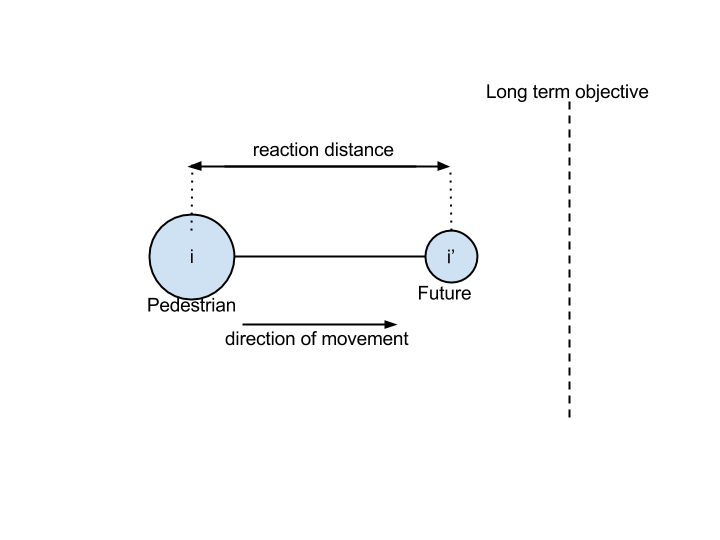
\includegraphics[scale=0.5]{pedestrian-top}\protect\caption{Vista superior de un peatón}
\end{figure}


Se reserva el uso de las letras para repersentar a un peatón y versión
con tilde para representar su future en el resto del documento.\\



\section{Funcionamiento}

Cada peatón en la simulación posee como objetivo final, alcanzar el
objetivo a largo plazo. Para asegurar esto, se trata siempre de mantener
al future (objetivo a corto plazo) alineado con el camino más corto
hacia el objetivo final. Sin embargo, pueden darse casos en donde
existan otros peatónes en esta trayectoria, obligando a tener que
utilizar rutas alternativas. Es en estas circunstancias es cuando
el objetivo a corto plazo va a ser trasladado según la situación. 

El movimiento de los peatónes se calcula en cuatro etapas: 
\begin{enumerate}
\item Cálculo de la fuerza sobre sobre cada future. 
\item Actualización de la posición de cada future. 
\item Cálculo de la fuerza sobre cada peatón. 
\item Actualización de la posición de cada peatón. \\

\end{enumerate}
En donde, cada etapa se define de la siguiente manera:
\begin{enumerate}
\item Cálculo de la fuerza sobre sobre cada future. 


En esta etapa, lo que se va a hacer es calcular la fuerza que sufre
cada uno de los futures existentes debido a la existencia de otros
peatónes. Esta se realiza sólo cuando la distancia entre el peatón
y su future se encuentra por encima de cierto valor. Esto es así ya
que a altos niveles de densidad de personas. Uno ya no puede moverse
y simplemente es arrastrado por la masa de gente.


En el caso contrario, cuando que un peatón se encuentra habilitado
para moverse, se realiza un filtro de todos aquellos peatónes que
se encuentran a sus espaldas, ya que estos no son casos que afectan
la trayectoria de la persona. La condición que debe cumplirse para
considerar un peatón $j$ como detrás del peatón $i$ es: 


\[
A=(Ax,\, Ay)=i
\]
\[
B=(Bx,\, By)=A+rotation(\overrightarrow{ii'},\,\pi/2)
\]
\[
C=(Cx,\, Cy)=j
\]
Luego, se debe cumplir que:


\[
(Bx-Ax)*(Cy-Ay)-(By-Ay)*(Cx-Ax)>0
\]



Una vez filtrados los peatónes, simplemente se calcula por cada future
restante, la fuerza de repulsión entre estos. Este se realiza utilizando
la fórmula: 


\[
F_{ext}(i)=\sum_{j}F_{i',j'}=\sum_{j}\alpha e^{-dist(i',j')/\beta}
\]



en donde $\alpha$ y $\beta$ son constantes predefinidas y fijas.
Los valores que se usaron son $\alpha=800$ y $\beta=[0.65,\,085]$
con distribución uniforme. Luego de calculadado $F_{ext}$, si su
valor es menor que cierto umbral, entonces se desprecia esta fuerza
y el future $i\lyxmathsym{\textquoteright}$ simplemente se alinea
con el objetivo estático a distancia que indique la distancia de reacción
del peatón. Caso contrario, cuando la contribución de las fuerzas
externas debe considerarse, se suma la contribución del peatón $i$
sobre su future para ajustarlo según su objetivo estático. Esta fuerza
se calcula a usando la formula del resorte. Los extremos de este resorte
se encuentran en el punto a distancia ``distancia de reaccion''
sobre el segmento de recta que une al peatón $i$ con su objetivo
estático y la posición del future $i'$.


A modo ilustrativo, se muestra en la figura 2 como la trayectoria
del peatón $i$ es afectada por la del peatón $j$ a través de $F(i',\, j')$
y es alineada al objetivo con $F(i,\, i')$


\begin{figure}[H]
\centering{}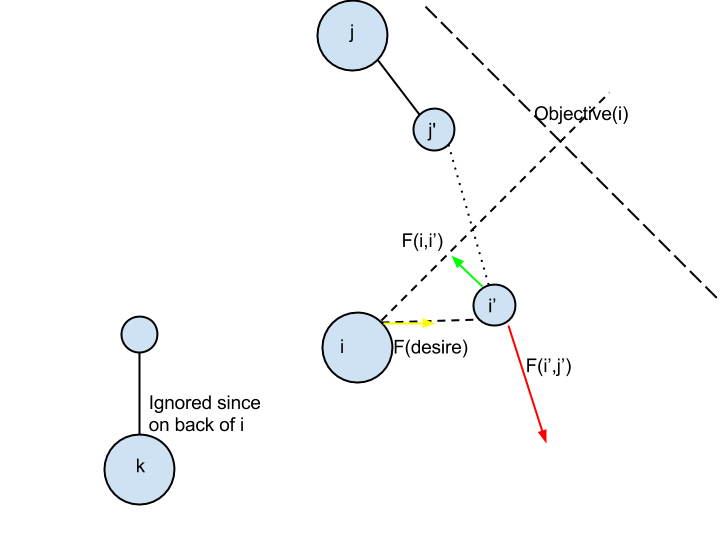
\includegraphics[scale=0.5]{pedestrian-top-forces}\protect\caption{Fuerzas que actúan sobre el Future $i'$}
\end{figure}

\begin{enumerate}
\item Actualización de la posición de cada future. 


En esta etapa, simplemente se actualiza la posición de cada future
según el cálculo de la fuerza $F$ aplicada en la etapa previa. Este
cálculo se realiza utilizando las fórmulas de Euler. 


Para romper con situaciones con altos grados de simetría, se agrega
ruido $P=10\%$ sobre $F$. Para esto, se aplican dos formas de ruido:
\begin{itemize}
\item Ruido longitudinal:

\begin{itemize}
\item Se toma un valor $p$ según una distribución aleatoria uniforme en
el intervalo $[-P,\, P]$ y se calcula: $FL_{i'}=F_{i'}*p$
\end{itemize}
\item Ruido angular:

\begin{itemize}
\item Se toma $sgn=\{-1,\,1\}$ utilizando una distribución uniforme y $p$
en $[-P,\, P]$ con la misma distribución. Luego se calcula: $FA_{i'}=rotation(F_{i'},\,\pi*sgn)*p$
\end{itemize}
\end{itemize}

Por último se toma $F'_{i'}=F_{i'}+FL_{i'}+FA_{i'}$ y de aplican
las ecuaciones de movimiento.

\item Cálculo de la fuerza sobre cada peatón. 


El peatón siempre se mueve hacia la dirección en la que apunta su
future y de acuerdo a la fuerza de deseo.


Esta fuerza representa la atracción que un peatón $i$ ejerce sobre
sí mismo a fin de dar un paso hacia su future y tratar de alcanzarlo.
Esta definida por la siguiente fórmula: 


\[
F_{deseo}=\frac{dist(i',i)}{dist_{react}}\frac{v_{desire}-v_{curr}}{\tau}\frac{i'-i}{|i'-i|}
\]



En donde $\tau=0.5$

\item Actualización de la posición de cada peatón. 


La nueva posicion de cada peatón es calculada en esta etapa utilizando
las mismas fórmulas mencionada en la etapa 2.

\end{enumerate}
\end{enumerate}

\section{Validación del modelo }

Los resultados obtenidos fueron comparados utilizando el modelo ``Social
Force Model'' utilizando los valores propuestos por Dirk Helbing
{[}2{]}. Los escenarios de prueba fueron cruce y hallway. 

Los resultados fueron cuantificados utilizando las siguientes métricas:
\begin{enumerate}
\item Cantidad total de colisiones


TODO: (como se calcula)

\item Duración promedio de las coliciones


TODO: (como se calcula)

\item Velocidad promedio de viaje


TODO: (como se calcula)

\item Tiempo promedio de viaje 


TODO: (como se calcula)

\item Promedio de la distancia recorrida 


TODO: (como se calcula)

\item Ángulo giro promedio


TODO: (como se calcula)

\end{enumerate}
\vspace{1cm}
En la tabla a continuación se presentan las mediciones de las métricas
utilizando un total de $10$ corridas:

\begin{tabular}{|c|c|c|c|c|c|c|}
\hline 
Valores & 1 & 2 & 3 & 4 & 5 & 6\tabularnewline
\hline 
\hline 
$\alpha=800,\,\beta=[0.65,\,0.85]$ & (1.800, 0.748)  & (34.600, 8.333)  & (1.024, 0.016)  & (1.910, 0.022)  & (2.392, 0.005)  & (111.062, 19.122)\tabularnewline
\hline 
$\alpha=2000,\,\beta=0.08$ & (5.333, 2.625) & (12.333, 8.340)  & (1.052, 0.003)  & (1.876, 0.003)  & (2.391, 0.002)  & (106.185, 13.778)\tabularnewline
\hline 
\end{tabular}

\textbf{// Poner Graficos indicando distancias y esquemas del future
y la particula. }


\section{Conclusiones}

\textbf{// agregar al final futuras opciones que se abren con este
trabajo}

\pagebreak{}


\section{Referencias}
\begin{itemize}
\item {[}1{]} ... Karamouzas ...
\item {[}2{]} ...Helbing ...\end{itemize}

\end{document}
